\documentclass[11pt]{article}
\usepackage{amssymb, amsthm, amsmath}
\usepackage{graphicx}
\usepackage{bm}
\usepackage{doublespace}
\usepackage[authoryear]{natbib}
\usepackage{times}
\usepackage{multirow}


\newcommand{\bbeta}{\bm{\beta}}
\newcommand{\beps}{\bm{\epsilon}}
\newcommand{\bX}{\bm{X}}
\newcommand{\bY}{\bm{Y}}
\newcommand{\bI}{\bm{I}}


\linespread{1} 
\topmargin= -.5in \oddsidemargin= 0in
\evensidemargin= 0in \textwidth=6.5in \textheight=9in

\begin{document}

\begin{center}
	{\Large {\bf ST 758 Project 2}}\\ \vspace{12pt}
	{\large {\bf Jessica Miller}}\\ \vspace{12pt}
	Nov. 10, 2016
	\vspace{5mm}
	\vspace{5mm}
\end{center}

\begin{flushleft}
	For this assignment, I focused on the two issues that would slow down the computation of the Gaussian log-likelihood: the locations and the matrix inverse. To reduce the number of locations, I created grids to approximate the given locations. To calculate the matrix inverse, I investigated two different methods in R.
	\newline
	\newline
	The more locations included, the larger the distance matrix and the longer it takes to compute the log-likelihood. To explore this, I identified a group of knots. Using knots is fairly common practice in spatial statistics to approximate a group of locations, even those that are clustered. The locations for this assignment are very grid-like and so using another grid of knots is not an extreme idea. For the group of 1024 locations, I used a grid evenly spaced by 0.5 units. For my initial calculations, I used a grid spaced as such for each group of locations, no matter the density of the locations. See Figure \ref{e:max} for the grid using for the 1024 locations.	
\end{flushleft}

\begin{figure}[h]\begin{center}
		\caption{The 1024 locations, plotted in black, and the grid used to approximate them, plotted in red.}\label{e:max}
		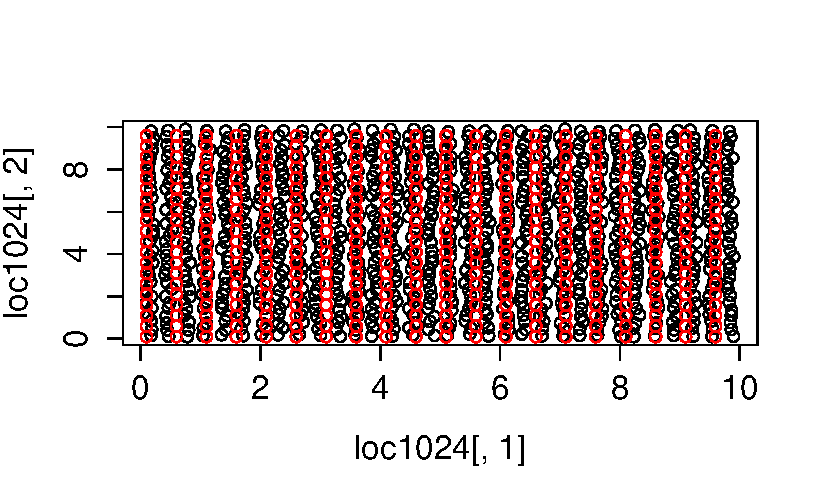
\includegraphics[width=.8\textwidth]{proj2_1}	
	\end{center}\end{figure}

\begin{flushleft}
	After I created my grids to approximate the locations, I continued to the calculation of the log-likelihood. I calculated two covariance matrices for each grid, following the equations from the project guidelines. From there, I focused on speed: how can I calculate the inverse of the covariance matrix, and thus the log-likelihood, the quickest? I investigated the timings using the \verb|solve()| and \verb|chol2inv()| functions in R. I generated 400 different multivariate Normal responses with mean 0 and sigma corresponding to the appropriate locations' covariance matrix. Using these, I calculated each log-likelihood and averaged their system speeds. In Table \ref{t:max}, we see that the \verb|chol2inv()| function calculates the inverse more quickly.
\end{flushleft}

\begin{table}[h]\caption{System timings (seconds) for each grid, covariance function, and matrix inversion method.}\label{t:max}	
	\begin{center}\begin{tabular}{ c || c || c c c  }
			Cov. Fun. & & 1024 & 2025 & 4096\\
			\hline
			Matern & solve & 0.077 & 0.087 & 0.088\\ & chol2inv & 0.036 & 0.040 & 0.040\\
			\hline
			Exp. & solve & 0.092 & 0.079 & 0.089\\ & chol2inv & 0.042 & 0.036 & 0.040\\ 
		\end{tabular}\end{center}\end{table}

\begin{flushleft}
	After this initial analysis of speed, I moved on to improving accuracy. I increased the density of the grids for the 2025 and 4096 locations. The 2025 locations were increased to a spacing of .375 units and the 4096 locations were increased to a spacing of .25 units to better approximate the original sites. The speed decreased significantly for the exponential covariance function, as seen in Table \ref{t:min}.
\end{flushleft}

\begin{table}[h]\caption{System timings (seconds) for the 2025 and 4096 grids, and each covariance function and matrix inversion method.}\label{t:min}	
	\begin{center}\begin{tabular}{ c || c || c c  }
			Cov. Fun. & & 2025 & 4096\\
			\hline
			Matern & solve & 0.079 & 0.089\\ & chol2inv & 0.035 & 0.041\\
			\hline
			Exp. & solve & 0.605 & 4.660\\ & chol2inv & 0.236 & 2.065\\ 
		\end{tabular}\end{center}\end{table}
		
\begin{flushleft}
	It is interesting that the Matern covariance function did not increase in timing as much as the exponential covariance function did. The \verb|chol2inv()| R function continued to calculate the inverse more quickly than the \verb|solve()| function.
	\newline\newline
	To optimize both speed and accuracy of the calculation of the Gaussian log-likelihood, I would use the higher grid densities when using the Matern covariance function and the lower grid densities when using the exponential covariance function. This promises the accuracy of the higher densities but the speed of the lower densities when using either covariance function.
\end{flushleft}


\end{document}
